\documentclass{abnt-UTFPR}                                          % estilo de documento abnTeX
\usepackage[alf,abnt-emphasize=bf,bibjustif,recuo=0cm]{abntcite}    % estilo de bibliografia abnTeX
\usepackage[brazil]{babel}                                          % pacote portugues brasileiro
\usepackage[latin1]{inputenc}                                       % pacote para acentuacao direta
\usepackage{amsmath,amsfonts,amssymb}                               % pacote matematico
\usepackage{graphicx}                                               % pacote grafico
\usepackage{times}                                                  % fonte times
\usepackage{verbatim}                                               % multi-line comment

% ---------- Preambulo ----------
\instituicao{Universidade Tecnol�gica Federal do Paran�} % nome da instituicao
\departamento{Departamento Acad�mico de Inform�tica} % nome do departamento
\programa{Bacharelado em Engenharia de Computa��o} % nome do curso

\documento{Trabalho de Conclus�o de Curso} % [Trabalho de Conclus\~ao de Curso] ou [Relat\'orio de Est\'agio]
\titulacao{Engenheiro} % [T\'ecnico], [Tecn\'ologo] ou [Engenheiro]

\titulo{An�lise Qualitativa de Algoritmos de Navega��o Fuzzy} % titulo do trabalho em portugues
\title{Qualitative Analysis of Fuzzy Algorithms} % titulo do trabalho em ingles

\autor{Alexandre Jacques Marin} % primeiro autor do trabalho
\autordois{J�lio Cesar Nardelli Borges} % segundo autor do trabalho, caso exista
\autortres{Yuri Antin Wergrzn} % terceiro autor do trabalho, caso exista
%\autorquatro{Nome do Quarto Autor} % quarto autor do trabalho, caso exista
\cita{MARIN, Alexandre; BORGES, J�lio; WERGRZN, Yuri } % sobrenome (maiusculas) e nome do(s) autor(es) do trabalho, separados por ponto-e-virgula (ate quatro autores para TCC)

\palavraschave{Navega��o, Fuzzy, Rob�s, Aut�noma, ...} % palavras-chave do trabalho
\keywords{Navigation, Fuzzy, Robots, Autonomous, ...} % palavras-chave do trabalho em ingles

\comentario{\UTFPRdocumentodata\ apresentado ao \UTFPRdepartamentodata\ como requisito parcial para obten\c{c}\~ao do grau de \UTFPRtitulacaodata\ no \UTFPRprogramadata\ da \ABNTinstituicaodata.}

\orientador{Jo�o Alberto Fabro} % nome do orientador do trabalho
%\orientador[Orientadora:]{Nome da Orientadora} % <- no caso de orientadora, usar esta sintaxe
\coorientador{Heitor Silv�rio Lopes} % nome do co-orientador do trabalho, caso exista
%\coorientador[Co-orientadora:]{Nome da Co-orientadora} % <- no caso de co-orientadora, usar esta sintaxe

\local{Curitiba} % cidade
\data{2012} % ano


%---------- Inicio do Documento ----------
\begin{document}

\capa % geracao automatica da capa
\folhaderosto % geracao automatica da folha de rosto
%\termodeaprovacao % <- ainda a ser implementado corretamente

% dedicat�ria (opcional)
\begin{dedicatoria}
Texto da dedicat\'oria.
\end{dedicatoria}

% agradecimentos (opcional)
\begin{agradecimentos}
Texto dos agradecimentos.
\end{agradecimentos}

% epigrafe (opcional)
\begin{epigrafe}
Texto da ep\'igrafe.
\end{epigrafe}

%resumo
\begin{resumo}
Este documento descreve detalhadamente a execu��o do projeto \"An�lise Qualitativa de Algoritmos de Navega��o Fuzzy\", feito como trabalho de conclus�o de curso de Engenharia de Computa��o na Universidade Tecnol�gica Federal do Paran�.
\end{resumo}

%abstract
\begin{abstract}
Abstract text (maximum of 500 words).
\end{abstract}

% listas (opcionais, mas recomenda-se a partir de 5 elementos)
\listadefiguras % geracao automatica da lista de figuras
\listadetabelas % geracao automatica da lista de tabelas
\listadesiglas % geracao automatica da lista de siglas
\listadesimbolos % geracao automatica da lista de simbolos

% sumario
\sumario % geracao automatica do sumario


%---------- Primeiro Capitulo ----------
\chapter{Introdu��o}

O problema do controle de navega��o de rob�s m�veis aut�nomos �
um campo da Engenharia da Computa��o que representa um grande
desafio, devido ao fato de o ambiente ser din�mico, haver sensoriamento
sujeito a ru�dos e exig�ncias de controle e tomada de decis�o em tempo
real. Um sistema de navega��o deve garantir que o rob� m�vel atinja
satisfatoriamente o destino de sua trajet�ria, enviando ao rob� os comandos
necess�rios para a sua locomo��o, de maneira precisa e suave, ao mesmo
tempo em que permite rea��es r�pidas �s mudan�as de ambiente para
evitar colis�es.
Na rob�tica m�vel, existem dois principais paradigmas que guiam os
projetos de diversas arquiteturas de sistemas de navega��o: o reativo e o
deliberativo. O paradigma reativo procura reproduzir a rea��o imediata dos
animais aos est�mulos do ambiente. Geralmente, arquiteturas reativas s�o
empregadas como uma camada de n�vel inferior na navega��o de rob�s
m�veis, pois apresentam a vantagem de resposta em tempo real uma vez
que mapeiam a leitura dos sensores, diretamente, em a��es. Arquiteturas
deliberativas, por outro lado, intercalam o processo da tomada de decis�o,
desde a percep��o at� a a��o, com uma etapa de planejamento a qual
demanda grande tempo computacional, impedindo a atua��o do rob� em
tempo real. Atualmente, s�o definidas arquiteturas h�bridas, conjugando
ambos os paradigmas\cite{FRACASSO}.
Ao realizar uma breve pesquisa para an�lise do estado da arte, foi poss�vel
perceber que existem v�rios trabalhos que apresentam novos m�todos
para navega��o aut�noma atrav�s do uso de l�gica Fuzzy. Entretanto,
n�o foi encontrado um trabalho propondo a compara��o entre m�todos
j� existentes. Com o intuito de preencher esta lacuna, a equipe optou
desenvolver este projeto.
Um dos modelos analisados neste trabalho � o modelo ED-FCM
proposto por Mendon�a no ano de 2010\cite{MENDONCA}. A sigla ED-FCM significa Event-
Driven Fuzzy Cognitive Maps e quer dizer Mapas Cognitivos Difusos
Dirigidos A Eventos.
Para realizar a compara��o pr�tica destes algoritmos, provou-se necess�ria uma
plataforma rob�tica, obtida atrav�s reconstru��o do rob� Bellator. O Bellator � um rob� m�vel que estava
em constru��o em outro projeto mas foi abandonado. Este rob�, sua reconstru��o
e adapta��o �s necessidades da equipe, � parte do projeto e � documentada em detalhes
neste documento. Esta adapta��o leva em conta
tamb�m a possibilidade de utiliza��o do Bellator para projetos futuros.
As principais motiva��es deste trabalho s�o o desenvolvimento de uma
plataforma rob�tica adequada para pesquisas acad�micas, tendo em
vista a falta de plataformas dispon�veis com este prop�sito, e o estudo de
sistemas de controle de navega��o rob�tica, que � um ramo de pesquisa
de elevado valor acad�mico. A possibilidade de disponibilizar uma nova
plataforma rob�tica para futuros estudos acad�micos e estudar um algoritmo
de navega��o pouco explorado s�o os maiores incentivos da equipe para a
realiza��o deste trabalho.

\section{Motiva\c{c}\~ao}

Uma das principais vantagens do uso do estilo de formata\c{c}\~ao {\ttfamily abnt-UTFPR.cls} para \LaTeX\ \'e a formata\c{c}\~ao \textit{autom\'atica} dos elementos que comp\~oem um documento acad\^emico, tais como capa, folha de rosto, dedicat\'oria, agradecimentos, ep\'igrafe, resumo, abstract, listas de figuras, tabelas, siglas e s\'imbolos, sum\'ario, cap\'itulos, refer\^encias, etc. Outras grandes vantagens do uso do \LaTeX\ para formata\c{c}\~ao de documentos acad\^emicos dizem respeito \`a facilidade de gerenciamento de refer\^encias cruzadas e bibliogr\'aficas, al\'em da formata\c{c}\~ao~-- inclusive de equa\c{c}\~oes  matem\'aticas~-- correta e esteticamente perfeita.

\section{Objetivos}

\subsection{Objetivo Geral}

Os principais objetivos do projeto s�o construir uma plataforma rob�tica est�vel cujo hardware e software
dever�o ser bem documentados, visando extensibilidade para projetos futuros, e utilizar-se desta plataforma para testar dois algoritmos de navega��o fuzzy, comparando-os segundo diversos crit�rios, tais como: tamanho e complexidade do c�digo, custo
computacional, tempo de resposta, efic�cia.

\subsection{Objetivos Espec\'ificos}

Os objetivos espec�ficos deste projeto remetem n�o apenas � an�lise de algoritmos de navega��o fuzzy mas tamb�m quanto � qualidade da re-constru��o da plataforma rob�tica. 
De maneira geral, a plataforma deve ser capaz de detectar
obst�culos pr�ximos a mesma atrav�s de sensores de dist�ncia, e dever� se deslocar por meio de um par de motores de corrente
cont�nua acoplados a rodas revestidas de borracha. As rodas devem ser equipadas com encoders para aux�lio � odometria. A
plataforma deve executar comandos de movimenta��o, os quais s�o:
transla��o para frente e para tr�s, e rota��o, no sentido hor�rio e anti
hor�rio. Um sistema microcontrolador deve processar os sinais dos sensores
de dist�ncia e dos encoders das rodas, e implementar rotinas de baixo
n�vel para acessar os dados dessa leitura. Esse sistema tamb�m deve
implementar rotinas de baixo n�vel para controlar a pot�ncia dos motores
e calcular deslocamento, velocidade e acelera��o linear e angular da
plataforma.
A plataforma deve ser extens�vel a qualquer outro sistema de
processamento. O microcontrolador desta deve implementar rotinas de
baixo n�vel para comunica��o de dados. A plataforma deve apresentar
interface de alto n�vel para leitura dos dados dos sensores e recebimento de
comandos de movimenta��o.
A documenta��o de hardware e software da plataforma deve atender
aos requisitos de um projeto de engenharia, incluindo: diagramas de blocos, diagramas esquem�ticos,
diagramas UML de classes, casos de uso, entre outros.
Os dois algoritmos de navega��o dever�o ser implementados em uma hardware acoplado � plataforma rob�tica, visando reduzir atrasos de comunica��o. Este hardware dever� ser capaz de ler os dados dos sensores do rob� como fonte de informa��es para os algoritmos e enviar comandos de movimenta��o ao mesmo.
Os testes dos algoritmos dever�o realizados inicialmente em um
ambiente aberto e livre de obst�culos, onde o rob� dever� deslocar-se em uma trajet�ria de
um ponto inicial a um ponto final com velocidade constante. Posteriormente,
o ambiente ser� limitado progressivamente, acrescentando-se obst�culos
entre os dois pontos da trajet�ria. Em cada caso, os dois algoritmos
ser�o experimentados sob as mesmas condi��es.

%---------- Estado inicial do Projeto ----------
\chapter{Estado do Projeto}
\label{chap:estpro}

Este cap�tulo visa descrever com quais recursos a equipe iniciou a execu��o do projeto, tanto materiais como imateriais. Ou seja, este cap�tulo descreve a situa��o do rob� e seus componentes f�sicos, o principal recurso material do projeto e, tamb�m, de seus componentes de software e a documenta��o dos mesmos, da forma como entregue � equipe no in�cio do projeto.

\section{Vis�o Geral}

O rob� disponibilizado � equipe para a realiza��o do projeto, o Bellator, � resultado de um projeto n�o conclu�do, visando a implementa��o de uma plataforma rob�tica controlada remotamente por joystick. Para tal, o rob� foi dividido em tr�s camadas: Baixo n�vel, Alto n�vel e Supervis�rio. A camada de baixo n�vel seria respons�vel por controlar os motores do rob�, bem como receber leituras dos sensores do mesmo. A camada de alto n�vel comunicaria-se com a camada de baixo n�vel via conex�o serial, faria obten��o de v�deo atrav�s de uma webcam e comunicaria-se com a camada supervis�ria atrav�s de uma conex�o sem-fio. Esta �ltima seria a interface com o usu�rio para realizar o controle remoto do rob�. O diagrama esquem�tico a seguir demonstra esta situa��o:

\begin{figure}[!htb]
	\centering
	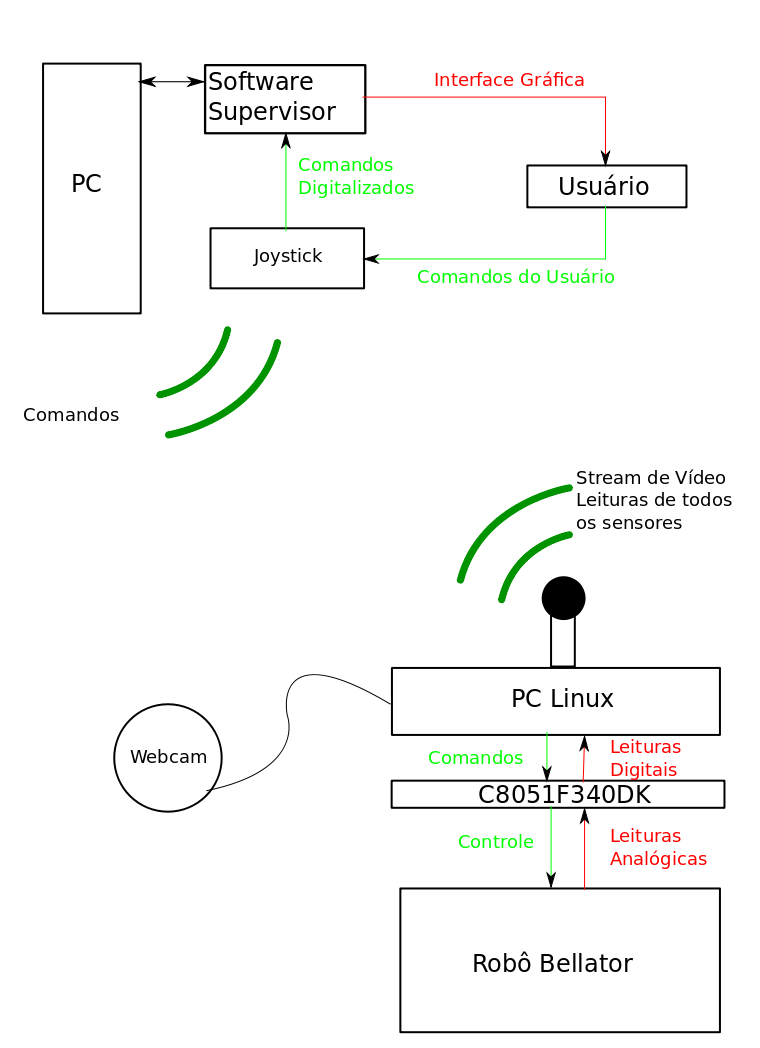
\includegraphics[width=\textwidth]{./figs/diagsis.png}
	\caption[Diagrama original do Bellator]{Diagrama original do projeto Bellator, retirado da monografia do mesmo.}
	\fonte{\cite{BELLATOR}}
	\label{fig:diagsis}
\end{figure}

A partir da figura \ref{fig:diagsis}, o funcionamento do projeto bellator pode ser analisado. A camada de baixo n�vel � composta pelo rob� bellator, equipado com dois motores el�tricos Bosch FPG 12V, seis sensores de dist�ncia "2Y0A02F98" da Sharp, uma bateria Unybatt 12V-7.2 Amp�re hora, duas pontes H e a placa micro-controlada C8051F340, capaz de ler e converter leituras de tens�o anal�gicas dos sensores do rob� bem como produzir sinais de controle para os motores do rob�. Esta placa est� conectada � camada de alto n�vel, composta por um PC Embarcado VIA EPIA ME60000 Mini-ITX com sistema operacional Linux, atrav�s de uma conex�o serial. Utilizando-se de um protocolo de comunica��o, este PC Embarcado envia comandos de movimenta��o para a camada de baixo n�vel e recebe as leituras dos sensores obtidas pela camada de baixo n�vel. O PC Embarcado tamb�m comunica-se com a camada de alto n�vel para receber comandos de movimenta��o do usu�rio e enviar as leituras dos sensores para o mesmo. Al�m disso, o PC Embarcado envia, tamb�m via comunica��o sem-fio, um stream de v�deo gerado por uma webcam Genius iLook 316. Finalmente, o software supervisor remoto, executado em um PC com m�quina virtual java, fornece as informa��es recebidas da camada de alto n�vel para o usu�rio, ajudando-o a tomar decis�es sobre a locomo��o do rob�. O software tamb�m recebe comandos de movimenta��o do usu�rio, gerados em um Joystick do videogame Sony Playstation 2, enviando-os para a camada de alto n�vel pela mesma conex�o.

O leitor pode observar desde j� que o projeto Bellator apresenta objetivos muito distintos do projeto "Algoritmos de Navega��o Fuzzy Uma An�lise Qualitativa". Assim, n�o ser� feita uma descri��o detalhada de todos os componentes do projeto bellator. A seguir, ser� descrito como o rob� foi recebido pela equipe e quais componentes foram re-aproveitados.

\section{Recebimento do Rob�}
\label{sec:recrobo}

O rob� Bellator foi entregue a equipe em abril de 2011, em uma caixa, desmontado, juntamente de toda a documenta��o dispon�vel do mesmo, por m�dia digital. A caixa continha os seguintes itens:

\begin{itemize}
\item Chassi do rob� Bellator com dois motores Bosch FPG12V e pontes H acoplados
\item Cinco sensores de dist�ncia "2Y0A02F98" da Sharp
\item Duas baterias Unybatt 12V-7.2 Amp�re hora
\item Uma placa micro-controlada C8051F340
\item Uma placa de roteamento, produzida pelo projeto Bellator
\item Um PC Embarcado VIA EPIA ME60000 Mini-ITX
\end{itemize}

O chassi do rob� e seus componentes acoplados s�o a base da plataforma rob�tica a ser utilizada pela equipe e cr�ticas para a execu��o do projeto. Os sensores de dist�ncia, um a menos que os dispon�veis no projeto Bellator, s�o essenciais para a localiza��o do rob� e de obst�culos, sendo cr�ticoos para o projeto, tamb�m. A placa micro-controlada tamb�m � um recurso cr�tico para o projeto pois � um componente respons�vel por todo o controle de baixo n�vel do rob� que, al�m disso, possui software reaproveit�vel e documentado. As baterias s�o um recurso necess�rio para o projeto, por�m s�o de f�cil acquisi��o, ao contr�rio dos outros componentes aqui citados. Elas foram testadas e uma das baterias apresentou defeito e foi substituida pela equipe. Visto a import�ncia destes elementos para o projeto, eles ser�o descritos em maiores detalhes no cap�tulo \ref{chap:esprob}, com apoio da documenta��o produzida pelo projeto Bellator.
Alguns itens mencionados na se��o anterior, referentes ao projeto Bellator, n�o foram recebidos ou n�o ser�o utilizados no novo projeto. A webcam e joystick mencionados na se��o anterior n�o foram entregues, pois n�o ser�o necess�rios para este projeto, visto que um sistema de navega��o autonoma n�o necessita de Joystick e, no caso deste projeto, n�o ser� capaz de utilizar-se de um stream de v�deo. A placa de roteamento ser� utilizada apenas como aux�lio para testes iniciais dos componentes do rob�, visto que � essencial para o funcionamento do rob�, embora seja muito rudimentar. Esta placa ser� reprojetada e reconstru�da. O PC Embarcado foi entregue destitu�do de qualquer documenta��o sobre os componentes de software do mesmo. Al�m disso, como o novo objetivo do rob� n�o necessita de comunica��o sem-fio e n�o utilizar� stream de v�deo, motivo principal para a utiliza��o deste PC no projeto anterior, a equipe optou por descartar este recurso do projeto e utilizar outra placa mais simples e menor, que ser� descrita em detalhes na se��o \ref{chap:esprob}.

A documenta��o dispon�vel � equipe, produzida pelo projeto Bellator, descreve em detalhes os componentes de hardware da plataforma rob�tica Bellator, do software de controle supervis�rio e da camada de baixo n�vel do rob�, ou seja, o software da placa C8051F340\cite{BELLATOR}. Esta documenta��o ser� utilizada como refer�ncia para o reaproveitamento da plataforma rob�tica, com exce��o da documenta��o referente ao software de controle supervis�rio, que n�o ser� utilizado.

\subsection{Teste dos Componentes}

Ap�s o recebimento do rob�, foram realizados testes para garantir a funcionalidade dos componentes recebidos, visto que a falha de alguns destes componentes poderiam implicar na impossibilidade de continuar o projeto ou em atrasos significativos. Estes testes tamb�m foram necess�rios para determinar de forma mais precisa o que poderia ser reaproveitado do projeto Bellator. De acordo com a documenta��o do projeto Bellator \cite{BELLATOR}, o rob� deveria ser capaz de, se montado conforme as instru��es na mesma, funcionar como um sistema controlado remotamente. A equipe optou por testar apenas a camada de baixo n�vel, como definida no projeto Bellator, isoladamente. O rob� foi montando utilizando-se do chassi e seus componentes acoplados, a placa de roteamento, a bateria e a placa C8051F340. Foi observado mal-funcionamento da placa de roteamento, que foi f�cilmente reparada atrav�s da troca de um transistor.

Com os componentes mais cr�ticos testados, a equipe tentou testar o PC Embarcado. Por�m, a aus�ncia de documenta��o sobre este documento impossibilitou o teste e, ap�s in�meras tentativas falhas de utiliza��o do mesmo, a equipe optou por n�o utilizar o PC Embarcado VIA EPIA ME60000 para o projeto, visando reduzir o crescente atraso causado por este. A camada supervis�ria do projeto Bellator n�o foi testada, visto que o rob� passar� a ser aut�nomo, n�o necessitando de uma camada supervis�ria. 

\chapter{L�gica Fuzzy}
Esta se��o tem como fun��o descrever o que � a l�gica fuzzy, como surgiu, como funciona e como projetar um sistema fuzzy.

A l�gica fuzzy � baseada no trabalho de Lofti Zadeh, que prop�s a teoria de conjuntos
fuzzy em 1965~\cite{FUZZYLOGIC}. Na teoria cl�ssica de conjuntos, um elemento tem seu
grau de pertin�ncia ao conjunto representado por uma vari�vel booleana, ou seja, ou o elemento
pertence ao conjunto ou n�o pertence. Num conjunto fuzzy, no entanto, um elemento tem seu grau
de pertin�ncia representado por um valor real no intervalo [0, 1].

Uma aplica�ao b�sica e cl�ssica da l�gica fuzzy � a classifica��o de uma vari�vel cont�nua. Por exemplo, 
se fosse necess�rio classificar um valor de temperatura, poderia ser utilizado um conjunto fuzzy com as vari�veis
FRIO, MORNO e QUENTE. Para saber a classifica��o de certo valor de temperatura, poderia ser utilizado algo
como o que est� representado na figura \ref{fig:fuzzyclasses}.

\begin{figure}[!htb]
    \centering
    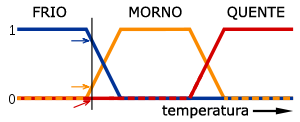
\includegraphics{./figs/fuzzyclasses.png}
    \caption[Classifica��o Fuzzy]{Classifica��o de valores de temperatura utilizando l�gica fuzzy.}
    \fonte{\cite{FUZZYLOGIC}}
    \label{fig:fuzzyclasses}
\end{figure}

A temperatura destacada na figura tem os seguintes graus de pertin�ncia: 0.8 FRIO, 0.2 MORNO e 0 QUENTE.
� comum tamb�m associar outras vari�veis lingu�sticas para caracterizar os valores. No caso do exemplo, uma associa��o
poss�vel seria: bastante frio, levemente morno, nada quente.

Com base na sa�da do classificador, um sistema fuzzy pode tomar decis�es. Por exemplo, caso o objetivo fosse controlar
a temperatura de uma caldeira, para deix�-la bem quente, a observa��o de que est� bastante frio implicaria
na necessidade da eleva��o da quantidade de energia disponibilizada para seu aquecimento. Conforme a temperatura subisse, novas observa��es seriam feitas e classificadas, levando a outras regula��es da fonte de calor, at� chegar � temperatura esperada. Quanto mais pr�ximo do n�vel esperado, menores as varia��es causadas na regula��o da fonte de calor.

As decis�es tomadas pelo sistema s�o definidas por um conjunto de regras fuzzy, cujo formato b�sico �:

SE X ENT�O Y

onde X � uma express�o contendo uma ou mais vari�veis lingu�sticas e Y a a��o a ser tomada. Retomando o exemplo da caldeira,
uma regra poss�vel seria: SE bastante frio ENT�O aumentar bastante o fornecimento de calor.

� evidente que os conceitos FRIO, MORNO e QUENTE s�o totalmente subjetivos (cada aplica��o tem par�metros espec�ficos).
O mesmo � v�lido para outras grandezas f�sicas, tais como: velocidade, dist�ncia, press�o, for�a, acelera��o etc.
Os valores e fun��es utilizadas para avaliar tais grandezas (algo como o modelo mostrado na figura \ref{fig:fuzzyclasses})
s�o determinados por quem est� desenvolvendo o sistema fuzzy, com os devidos ajustes para melhor adequa��o � aplica��o em
quest�o. Da mesma forma, as decis�es a serem tomadas com base nos dados classificados s�o definidas pelo usu�rio. Isso �
interessante quando se considera a adi��o de novos sensores e, consequentemente, novos dados. Uma simples altera��o ou adi��o
de novas regras � o suficiente para adaptar o sistema �s novas entradas.



Pelo fato de permitir a classifica��o de dados de uma forma mais flex�vel (em compara��o com a teoria cl�ssica de conjuntos),
os dados de entrada para um sistema fuzzy n�o precisam ser t�o precisos, sem ru�dos, j� que a presen�a de ru�dos
causaria apenas pequenas varia��es na classifica��o (enquanto numa classifica��o bin�ria um n�vel baixo de ru�do pode
mudar uma classifica��o totalmente, ao passar um limite pr�-definido).

Para projetar um sistema fuzzy, o seguinte conjunto de passos pode ser seguido~\cite{FUZZYLOGICTUTORIAL}:

\begin{enumerate}
    \item Defini��o do que vai ser controlado, com quais crit�rios, qual o tipo de sa�da desejado.
    \item Determina��o da rela��o entre a entrada e a sa�da, escolha do n�mero de vari�veis de entrada para o sistema.
    \item Utilizando a estrutura de regras da l�gica fuzzy, dividir o problema principal em v�rias tarefas menores. Estas
    regras devem descrever o comportamento desejado conforme definido no item 1. O n�mero e complexidade das regras depende do n�mero de par�metros de entrada a serem processados e do n�mero de vari�veis fuzzy associadas aos mesmos.
    \item Cria��o das fun��es de classifica��o, que definem os significados (comumente atrav�s de vari�veis lingu�sticas)
    dos valores de entrada e sa�da. As sa�das das fun��es de classifica��o ser�o utilizadas nas regras
    \item Cria��o das fun��es para pr� e p�s-processamento necess�rias (para tratamento dos dados de entrada e sa�da)
    \item Testar o sistema, avaliar os resultados, ajustar as regras e fun��es de classifica��o. Repetir este passo
    at� obter um comportamento satisfat�rio.
\end{enumerate}




\chapter{Mapas Cognitivos Fuzzy}

Esta se��o tem como objetivo explicar o que s�o mapas cognitivos fuzzy, tamb�m conhecidos como FCM (Fuzzy Cognitive Maps), abordando o conceito, a estrutura, as propriedades e vantagens desse modelo, apresentar exemplos, descrever uma metodologia para constru�-lo e uma metodologia de aprendizado de m�quina em sistemas inteligentes utilizando FCM.

O modelo FCM � abordado na tese de doutorado de \cite{FCMENDONCA}. Mapas cognitivos s�o diagramas que representam liga��es entre palavras, id�ias, tarefas ou outros itens ligados a um conceito central, em volta do qual os elementos s�o dispostos radialmente e de forma intuitiva, de acordo com a import�ncia dos conceitos. Um mapa cognitivo pode ser tratato matematicamente por meio de opera��es com matrizes e baseado na teoria de grafos. Desse modo, cren�as ou afirma��es a respeito de um dom�nio de conhecimento limitado s�o expressas por palavras ou express�es lingu�sticas, interligadas por rela��es de causa e efeito. Esse modelo prop�e uma organiza��o de id�ias onde � poss�vel predizer as consequ�ncias que essa organiza��o implica ao universo representado, sendo considerado um modelo matem�tico da "estrutura de cren�as". O mapa cognitivo fuzzy � gerado quando se incluem a essa estrutura incertezas atrav�s da l�gica Fuzzy.

A estrutura de um mapa cognitivo fuzzy � um grafo direcionado, figura \ref{fig:fcm}, em que os valores num�ricos s�o vari�veis ou conjuntos fuzzy, os "n�s" s�o conceitos lingu�sticos, representados por conjuntos fuzzy e cada "n�" � associado a outros atrav�s de conex�es, a cada qual est� associado um peso num�rico, o qual representa uma vari�vel fuzzy relacionado ao n�vel de causalidade entre os conceitos.

\begin{figure}[!htb]
    \centering
    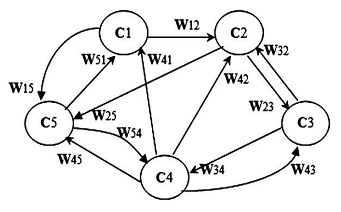
\includegraphics{./figs/fcm.png}
    \caption[Mapa Cognitivo Fuzzy]{Exemplo de um FCM (grafo).}
    \fonte{\cite{FCMENDONCA}}
    \label{fig:fcm}
\end{figure} 



\chapter{Conclus�o}

O presente trabalho de conclus�o de curso apresentou objetivos abrangentes, envolvendo desenvolvimento de hardware e software. No contexto da navega��o rob�tica, surgiu a necessidade de se utilizar um rob� real com a finalidade de se obter resultados mais significativos. Desse modo, foi elaborado um projeto cujo escopo tamb�m foi reconstruir e adequar uma plataforma rob�tica previamente dispon�vel, que � descrita na sec��o \ref{sec:estpro}, por�m que n�o estava em condi��es de uso imediato. A equipe procedeu com testes em laborat�rio de eletr�nica afim de avaliar as condi��es iniciais do rob�, conforme � descrito na sec��o \ref{sec:testecomp}. Uma an�lise de software foi efetuada e o c�digo original do microcontrolador C8051F340DK, disponibilizado como parte integrante do rob� Bellator \cite{BELLATOR}, foi avaliado e reconfigurado de acordo com as necessidades do projeto, o que � descrito em detalhes na se��o \ref{sec:codmicro}. Havendo necessidade de implementa��o de hardware, a equipe projetou e construiu uma placa de roteamento para alimentar os sensores e encoders, assim como tratar os sinais destes e os de PWM, como � descrito na se��o \ref{sec:desroteamento}. Finalmente, o hardware acoplado foi configurado e o software que executou os algortimos de navega��o foi desenvolvido, conforme a se��o \ref{sec:ts}. Com isso, a equipe concluiu a primeira parte do projeto, a qual consistiu na reconstru��o e adequa��o do rob� Bellator.

Estando a plataforma rob�tica funcional, seguiram-se o projeto e implementa��o dos algoritmos de navega��o propostos. A L�gica Fuzzy foi estudada e apresentada na se��o \ref{sec:logfuzzy} e a metodologia de Mapas Cognitivos Fuzzy (FCM) foi estudada e apresentada na se��o \ref{sec:fcm}. Com a teoria fundamentada, a equipe projetou os algoritmos e implementou-os na linguagem C++, compilados para executar no hardware acoplado, placa TS-7260. O projeto e a implementa��o dos algoritmos de navega��o Fuzzy e FCM s�o descritos em detalhes nas se��es \ref{sec:algfuzzy} e \ref{sec:algedfcm}, respectivamente. Ap�s a implementa��o, a equipe submeteu os algoritmos a uma s�rie de testes b�sicos, denominada Testes Iniciais, que serviram para fornecer a primeira realimenta��o do projeto dos algoritmos e pode ser lido na se��o \ref{sec:testesini}. Finalizados esses testes, foram elaborados testes complexos, denominados Testes Avan�ados, para estressar os sistemas de navega��o propostos e fornecer a segunda realimenta��o do projeto dos algoritmos, conforme � descri��o na se��o \ref{sec:testesavan}. Finalmente, ap�s os testes avan�ados, os algoritmos resolviam problemas complexos de navega��o, como o corredor sem sa�da e o problema de decis�o quando dois obst�culos laterais e um frontal era colocado diante do rob�, e poderiam ser usados nos testes finais, que forneceram os dados para a an�lise de resultados e foram denominados Testes Comparativos, conforme � descrito na se��o \ref{sec:testescomp}. Com isso foi conclu�do outros dois objetivos do projeto, que foram o projeto e implementa��o dos algoritmos de navega��o e a elabora��o e execu��o de uma metodologia de testes comparativos entre os algoritmos.

Para trabalhos futuros utilizando a plataforma Bellator reconstru�da, a equipe recomenda combinar sensores de ultra-som ao sensores infra vermelho, justificando isso porque os sensores de ultra-som apresentam uma faixa de opera��o cuja dist�ncia m�nima � menor que a do infra-vermelho, podendo capturar dist�ncias de 2 cm. Atualmente a dist�ncia m�nima suportada pelo sistema de navega��o � de 15 cm, com os sensores de ultra-som, os algoritmos poderiam operar em uma faixa mais abrangente. Outra sugest�o � introduzir ao sistema uma realimenta��o por b�ssola pois nesse projeto a realimenta��o odom�trica fornecida pelos encoders � utilizada para ajustar a velocidade das rodas e n�o faz uma interpreta��o da dire��o do rob�. Para tornar o rob� seguro para o manuseio, sugere-se a fixa��o dos sensores parafusando-os no chassi do Bellator e acoplando uma casca que proteja os circuitos microcontrolados. A equipe tamb�m recomenda a reconstru��o da placa de roteamento utilizando um m�todo industrial para confecc��o de placas de circuito impresso. Para os sistemas de navega��o, um trabalho futuro de grande riqueza seria introduzir ao sistema a capacidade de interpretar a posi��o do rob� em rela��o a um referencial. Com isso, o rob� seria capaz de resolver problemas nos quais este deve partir de um ponto inicial no espa�o a um ponto final, guiando-se pelos sensores para evitar colis�es e realimentar-se por um sistema de posicionamento para corrigir a traget�ria. Outro trabalho, produto deste, seria introduzir ao sistema uma mem�ria a qual pudesse mapear os obst�culos capturados pelos sensores do rob�, assim sendo, produzir-se-ia um artefato aut�nomo capaz de mapear terrenos. Outro aprimoramento da plataforma seria implementar um sistema de controle remoto por joystick, na qual uma base remota podesse pilotar o rob� via joystick. Finalmente, a equipe sugere um projeto futuro no qual seja implementado um sistema de vis�o computacional por c�mera de v�deo.

A equipe concluiu esta monografia justificando que os objetivos descritos na introdu��o, se��o \ref{rec:obj}, foram alcan�ados e est�o de acordo com os requisitos m�nimos de um curso de Engenharia de Computa��o. Os problemas encontrados na execu��o do projeto est�o associados ao escopo abrangente do mesmo, o qual envolveu o desenvolvimento de hardware e software em um projeto integrador. A subdivis�o do projeto em diversos objetivos, sendo um pr�-requisito para o outro, foi inevit�vel para alcan�ar os resultados finais. A equipe encontrou dificuldades durante a reconstru��o do rob�, configura��o da placa TS-7260, testes integrados de funcionamento do rob�, implementa��o dos algoritmos, execu��o dos testes dos algoritmos e an�lise de resultados. Durante a recontru��o, os componentes eletr�nicos foram testados isoladamente e houve riscos de haver danos, o que representaria atrasos no projeto. A placa TS-7260 apresentou complexidade para ser configurada pois n�o houve um t�cnico dispon�vel para auxiliar a equipe, a qual teve que aprender a trabalhar com esse hardware. Nos testes de integra��o da C8051F340DK e da TS-7260, que determinaram o funcionamento da plataforma rob�tica, foi exigido processos de depura��o integrados, nos quais os problemas foram isolados e corrigidos repetidas vezes. A implementa��o dos algoritmos at� a vers�o final, que foi utilizada nos testes comparativos, foi realizada paralelamente aos testes b�sicos e avan�ados, nas quais os problemas de navega��o foram detectados, isolados e corrigidos repetidas vezes. A metodologia de testes escolhida foi elaborada pela equipe e foram efetuados v�rios experimentos com registro em v�deo at� que se atingessem os resultados finais. Tendo com base os v�deos gravados e a experi�ncia em campo observada, a equipe precisou analisar os resultados, discut�-los e extrair conclus�es para finalizar o projeto, sendo que essa tarefa representou um trabalho cient�fico. 


%---------- Referencias ----------
\bibliography{reflatex} % geracao automatica das referencias a partir do arquivo reflatex.bib


%---------- Apendices (opcionais) ----------
\apendice
\chapter{Nome do Ap\^endice}

Use o comando {\ttfamily \textbackslash apendice} e depois comandos {\ttfamily \textbackslash chapter\{\}}
para gerar t\'itulos de ap\^en-dices.


% ---------- Anexos (opcionais) ----------
\anexo
\chapter{Nome do Anexo}

Use o comando {\ttfamily \textbackslash anexo} e depois comandos {\ttfamily \textbackslash chapter\{\}}
para gerar t\'itulos de anexos.

\end{document}
 